\documentclass[11pt, letterpaper]{article}
\usepackage[margin=0.5in]{geometry}
\usepackage{graphicx}
\usepackage{hyperref}
\usepackage{float}
\usepackage{amsmath}

\makeatletter
\newcommand{\university}[1]{\def\@university{#1}}
\newcommand{\prof}[1]{\def\@prof{#1}}
\newcommand{\course}[1]{\def\@course{#1}}
\def\@university{}
\def\@prof{}
\def\@course{}
      
\renewcommand\maketitle{
{\raggedright
\begin{center}
{\Large \@title }\\[1ex] 
{\@author }\\[1ex]
{\@university }\\[3ex]
{\@course}\\[1ex]
{\@prof }\\[1ex]
\@date\\[8ex]
\end{center}}}
\makeatother

\begin{document}

\title{Discovering and Characterizing MicroDNA in a Cancer Cell Line}
\author{Vincent Bowen}
\university{University of Colorado Boulder}
\course{CSCI 4444: Computational Genomics}
\prof{Dr. Ryan Layer}
\maketitle


\section{Introduction}
Circular DNA, particularly microDNA, have recieved significant attention for its potential role in genomic instability, cancer progression, and gene regulation. MicroDNA are short, circular DNA molecules that originate from the nuclear genome and have been detected in a variety of cell types, including cancerous tissues. Despite their prevalence, their formation mechanisms and biological functions remain poorly understood. 

This analysis presents a computational pipeline designed to detect and characterize microDNA using high-throughput sequencing data. The approach involves identifying soft-clipped reads from a BAM file, aligning these clipped sequences to one another and to a reference genome, and computing a scoring metric to evaluate the likelihood of circularization. Additionally, the performance of various pairwise sequence alignment algorithms was empirically compared to identify the most suitable tool for this task. MicroDNA events were manually verified, to ensure the accuracy of the report. This work aims to streamline the discovery of microDNA and provide a reproducible framework for further experimental testing with alternative genomes.


\section{Results}
A list of potential circles (microDNA) are written to a user-specified output file. If the output file is designated with a \verb|.csv| or \verb|.tsv| extension, the report includes the Start Position, End Position, Soft-Clip Alignment Score, Starting Soft-Clip Reference Alignment Score, Ending Soft-Clip Reference Alignment Score, and a computed Evidence Score for each candidate. Alternatively, if the user specifies a \verb|.txt| output, the report is expanded to include the full alignment strings: the alignment between the start and end soft-clips, the alignment between the start soft-clip and the reference genome, and the alignment between the end soft-clip and the reference genome. The reports are sorted by the Evidence Score, with the highest being first, and the lowest being last. 

$979$ candidate circles were generated, with $139$ having strong supporting evidence (a positive Evidence Score) using the provided BAM and FASTA files (See the \href{}{data} directory). The other potential circles were included to allow the user to validate circles manually using \href{}{IGV} if desired. A sample of both file classes can be seen in Figures~\ref{fig:txt_ex} and~\ref{fig:csv}

\begin{figure}[H]
\centering
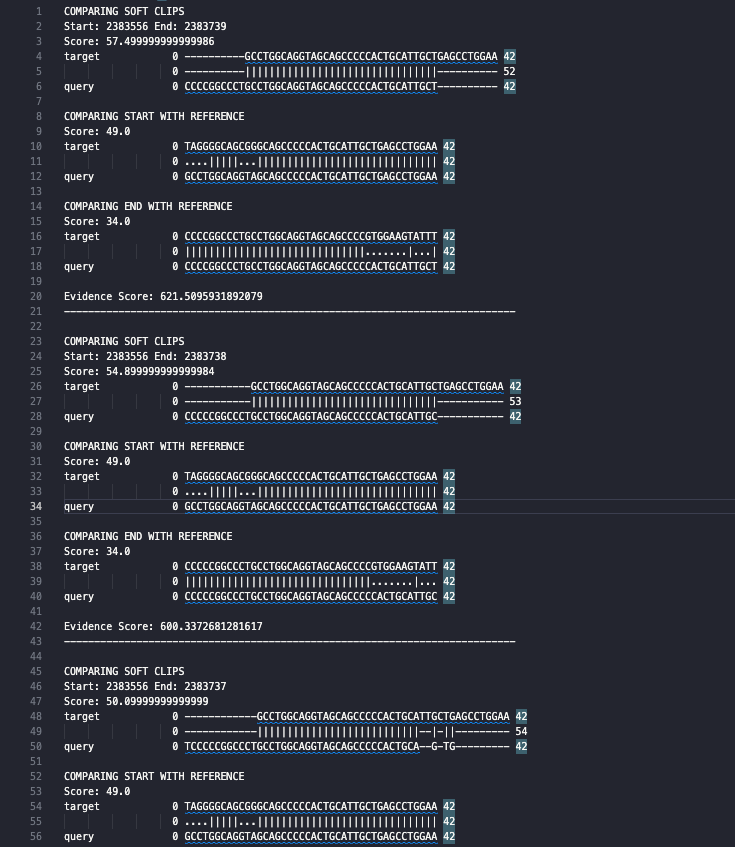
\includegraphics[width=0.6\textwidth]{imgs/txt_ex.png}
\caption{Sample of Text File Report}
\label{fig:txt_ex}
\end{figure}

\begin{figure}[H]
\centering
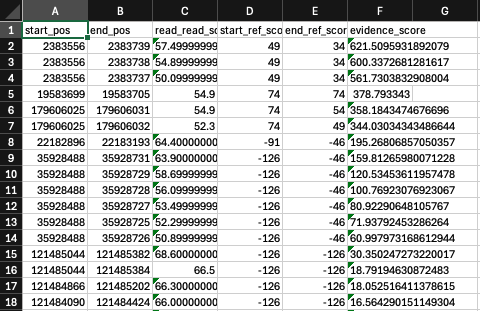
\includegraphics[width=0.75\textwidth]{imgs/csv_ex.png}
\caption{Sample of Comma Separated Value Report}
\label{fig:csv}
\end{figure}

Using the \verb|.txt| file containing the actual alignments, true circularization events could be manually verified. These potential circles were additionally hand validated in IGV by loading the FASTA and BAM file, then analyzing the sequence at the start position, and comparing that to the sequence at the end position.

\section{Methods}
\subsection{Performance of Pairwise Sequence Aligners}
After quickly observing substantial performance bottlenecks with the developed Smith-Waterman algorithm, the performance of various sequence aligners was tested. Four Pairwise Sequence Aligners were compared, with their performance recorded in Figure~\ref{fig:pw_performance}. The query size was set to 42 base pairs long, to simulate alignment on BAM reads with increasing target lengths. The empirical time to run each algorithm was recorded.

\begin{figure}[H]
\centering
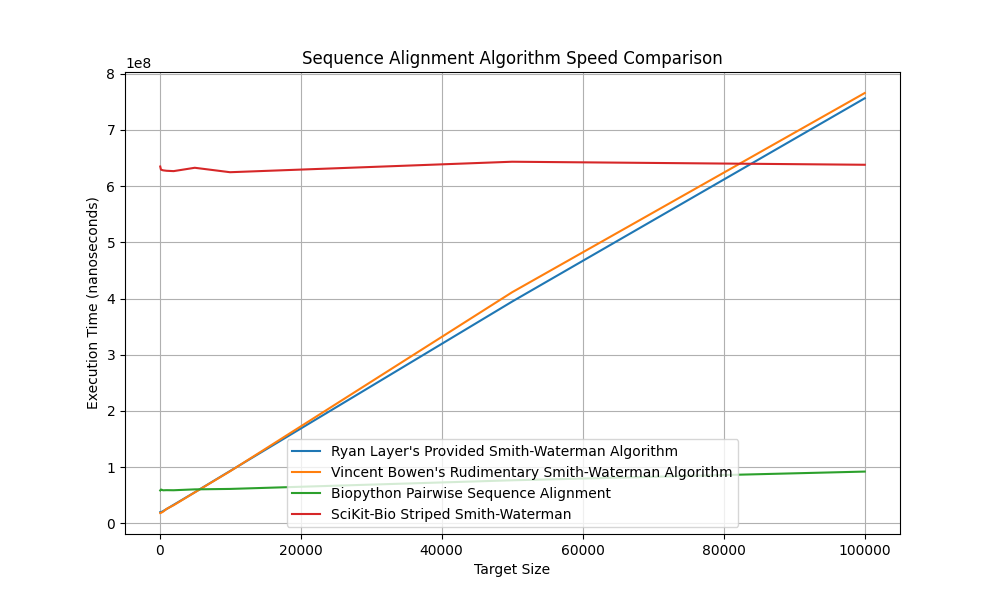
\includegraphics[width=0.75\textwidth]{imgs/pw_perf.png}
\caption{Performance of Various Pairwise Aligner Algorithms}
\label{fig:pw_performance}
\end{figure}

Four algorithms were tested:
\begin{enumerate}
    \item \href{google.com}{Ryan Layer's Smith-Waterman Algorithm}: Basic Python implementation using a fill matrix and traceback. 
    \item Vincent Bowen's Smith-Waterman Algorithm: Basic Python implementation, almost identical to the algorithm developed by Ryan.
    \item \href{https://scikit.bio/docs/dev/generated/skbio.alignment.StripedSmithWaterman.html}{Sci-Kit Bio's Striped Smith-Waterman Algorithm}: Python library performing a striped (banded) Smith Waterman Alignment.
    \item \href{https://biopython.org/docs/dev/Tutorial/chapter_pairwise.html}{Biopython's Pairwise Aligner}: Highly configurable Python library, automatically selecting between: Needleman-Wunsch, Smith-Waterman, Gotoh (three-state), and Waterman-Smith-Beyer global and local pairwise alignment algorithms, and the Fast Optimal Global Alignment Algorithm (FOGSAA) based on user-inputted scoring schema. For this experiment, the Gotoh algorithm was used.
\end{enumerate}

The algorithms developed by Vincent and Ryan exhibited nearly identical performance, which can be attributed to the fact that Vincent's implementation was derived from Ryan's methodology and reference materials. Both approaches demonstrated suboptimal performance when applied to larger targets due to a steep linear increase with respect to target length. The SciKit-Bio alignment algorithm showed unexpectedly poor performance on shorter target sequences—a notable limitation given that the majority of experimental targets were approximately 42 base pairs in length. In contrast, Biopython’s Pairwise Aligner exhibited marginally lower performance on extremely short targets but rapidly outperformed the other algorithms as target size increased. Notably, the linear growth rate of Biopython’s computational cost was significantly smaller compared to the Vincent and Ryan's algorithm.

Due to the superior performance of Biopython's implementation and its extensive configurability, it was selected as the alignment tool. A key advantage lies in the fine-grained control over alignment parameters, including direct specification of the alignment algorithm itself and the scoring schema. Parameters such as: mode, match score, mismatch score, gap opening score, and gap extension score can be individually adjusted. Furthermore, for soft-clipped sequences, additional control is available through the left and right query gap opening scores, as well as the left and right query gap extension scores. This level of specificity was preferred to the more limited configuration options—restricted to basic: gap, mismatch, and match penalties in the algorithms developed by Vincent and Ryan.

\subsection{Detection of MicroDNA}
To detect microDNA, an algorithm was developed to: identify circular DNA sequences, aggregate candidate findings, and compute a quantitative metric reflecting the strength of evidence for true circularization.

The steps of the algorithm are as follows:
\begin{enumerate}
    \item Load and process the \href{}{BAM} file to extract aligned sequencing reads and the \href{}{FASTA} file to serve as the reference genome for downstream analysis.
    \item Identify soft-clipped regions at the start and end of reads by analyzing the CIGAR strings for the presence of matching segments adjacent to soft-clips.
    \item Aggregate start and end soft-clips based on their genomic positions, recording the number of reads exhibiting these characteristics at each site.
    \item Apply an empirically defined threshold to determine high-support sites. In this study, a minimum of 10 supporting reads at a given position was required for further analysis. All other sites were filtered out.
    \item Perform an brute-force pairwise alignment between all identified starting and ending soft-clips to evaluate potential circular junctions. 

    Here the alignment was performed using the Gotoh algorithm with the following parameters: a match score of 2, a mismatch penalty of -2, a gap opening penalty of -1, and a gap extension penalty of -0.5, configured in global alignment mode. Additionally, the aligner was configured with minimal penalties for gap opening and extension at the ends of the query: the left and right query gap opening scores, and the left and right gap extension scores were all set to -0.1. This schema prefers shifting the position of the sequences versus a mismatch, a desirable property when identifying regions of central homology, and matching junction tags. 
    \item Compute an evidence-based metric to quantify the likelihood that a given candidate represents true microDNA (circle) formation. This score was defined as follows.
    \item Retain candidate pairs with an alignment score of at least 50 and a minimum separation of 5 base pairs between the clipped regions to ensure sequence homogeneity between the junction tags. These candidate sequences are then aligned against the reference genome. 
    
    Here the alignment was performed using the Gotoh algorithm with the following parameters: a match score of 2, a mismatch penalty of -3, a gap opening penalty of -25, and a gap extension penalty of -6, configured in global alignment mode. This schema strongly penalized both gap opening and extension, encouraging the aligner to favor mismatches instead. This behavior is desirable when aligning soft-clipped sequences, which are expected to differ from the reference genome at the soft-clipped regions, but should not be shifted through gap creation. This preserves the positional integrity of the sequences.
    \item Compute an evidence-based metric to quantify the likelihood that a given candidate represents true microDNA (circle) formation. This score was defined as follows.
    \begin{align*}
        Score &= \frac{(SCAS * 8 + SSCRAS * 2 + ESCRAS * 2)}{Penalty}\\
        &\text{Where, }\\
        Penalty &= ((span - 200) / 200) ** 2 + 1 \\
    \end{align*}
    Additionally, $SCAS$ is the Soft-Clip Alignment Score, the score between the start and end soft-clips, $SSCRAS$ is the Starting Soft-Clip Reference Alignment Score, the score between the start soft-clip and the reference genome, and $ESCRAS$ is the Ending Soft-Clip Reference Alignment Score, the score between the ending soft-clip and the reference genome. Arbitrary but empirically motivated weights were applied to these scores to emphasize the alignment between the soft-clips themselves ($SCAS$), as this was observed to be a strong indicator of circularization.
    
    A $Penalty$ term was also introduced, defined as a quadratic function that rewards a homologous span close to 200 base pairs. This design penalizes extremely short or excessively long regions of homology, which are unlikely to represent true circular DNA junctions based on empirical observations.
    \item Sort the candidates based on the defined metric, and write to a user-defined .txt, .csv, or .tsv file.
\end{enumerate}

\subsection{Reproducibility}

To replicate these experiments, clone the repository and then run the
experiments and analysis as follows:
\begin{verbatim}
$ git@github.com:vincedbowen/micro-dna.git
$ cd micro-dna
\end{verbatim}
\begin{enumerate}
    \item Pairwise Aligner Performance Test 
    \begin{verbatim}
    $ cd pairwise-aligner-comparer
    $ python compare_pwa.py
    \end{verbatim}
    \item MicroDNA Analysis
    \begin{verbatim}
    $ cd micro-dna-finder/cli
    $ python3 main.py \
      -bf ../data/SRR413984.sorted.NC_000001.10.bam \
      -ff ../data/GCF_000001405.13_GRCh37_genomic.NC_000001.10.fna \
      -of ../results/results.<file-extension>
    \end{verbatim}
    Where file-extension is \verb|txt|, \verb|tsv|, or \verb|csv|.
\end{enumerate}

\end{document}
